%!TEX root = thesis.tex

%:-------------------------- Preamble -----------------------

% Three languages are supported, which will be reflected in the logo on the front page. Pass the appropriate language
% specified as a class option to uit-thesis. Passing any other languages supported by babel will result in the default
% language on the frontpage. If no language is passed, the default is selected.
%  - USenglish (default)
%  - norsk
%  - samin
% The frontpage comes in two variants, Master's thesis and PhD. Master is default, use classoption 'phd' for the PhD version.
\documentclass[USenglish]{uit-thesis}

% Lorem ipsum
%\usepackage{lipsum}

\makeglossaries

% Add external glossaryentries
\loadglsentries{acronyms}
\newacronym{api}{API}{application programming interface}\glsunset{api}
\newacronym{2api}{2API}{application programming interface}
\newacronym{d3}{D3}{Data-Driven Documents}
\newacronym{html5}{HTML5}{version 5 of the HyperText Markup Language standard}
\newacronym{wsn}{WSN}{Wireless Sensor Network}
\newacronym{bs}{BS}{Base Station}
\newacronym{ch}{CH}{Cluster Head}
\newacronym{coat}{COAT}{Climate-ecological Observatory for Arctic Tundra}


\newglossaryentry{thesis}
{
  name=thesis,
  description={is a document submitted in support of candidature for an
    academic degree or professional qualification presenting the author's research and findings},
}
\newglossaryentry{lage}
{
  name={long ass glossary entry},
  description={is a long ass entry with a lot of text describing the properties of the glossary entry. Hopefully this spans some lines now.},
}


\newcommand{\listdefinitionname}{My list of definitions}
\newlistof{definition}{def}{\listdefinitionname}
\newcommand{\definition}[1]{%
  \refstepcounter{definition}%
  \par\noindent\textbf{The Definition~\thedefinition. #1}%
  \addcontentsline{def}{definition}
    {\protect\numberline{\thechapter.\thedefinition}#1}\par%
}

\begin{document}

%:-------------------------- Frontpage ------------------------

\title{Peer Observations of Observation Units}
%\subtitle{Subtitle}			% Optional
\author{Camilla Stormoen}
\thesisfaculty{Faculty of Science and Technology \\ Department of Computer Science}
\thesisprogramme{INF-3981 Master's Thesis in Computer Science ... May 2018}
%\ThesisFrontpageImage{example_image.jpg}	% Optional

\maketitle

%:-------------------------- Frontmatter -----------------------
\frontmatter

%\begin{dedication}
%To Leslie.
%Fuck you very much.
%\end{dedication}


%\begin{epigraph}
%\epigraphitem{Simplicity is prerequisite for reliability.}{Edsger Dijkstra}
%\epigraphitem{Beware of bugs in the above code;\\I have only proved it correct, not tried it.}{Donald Knuth}
%\end{epigraph}


\begin{abstract}
What is wrong with the world? Motivation 1-3 sentences, Arch, Des, Imp, Exp 1,2-3 sentences, results and main conclusion.
\end{abstract}

\begin{acknowledgement}
\iffalse
First I would like to thank my main advisor Professor Otto Anshus and co-advisor Associate Professor John Markus Bjørndalen for providing guidance, support, ideas and feedback whenever I needed it through this thesis.

I want to express my sincerest gratitude to the \textit{Masterinos}. I would not have made it without you guys. 

I would also like to thanks my parents for encouraging me to take a higher education and supporting me through every decision. A great thanks to my boyfriend
\fi
\end{acknowledgement}

\tableofcontents

%\listofdefinition

%\listoflistings

\printglossary
%\printglossary[type=\acronymtype]
%\printglossaries


%:-------------------------- Mainmatter -----------------------
\mainmatter

\chapter{Introduction}
\textbf{FRA CAPSTONE:}
The Arctic tundra in the far northern hemisphere is challenged by climate changes in the world today and is one of the ecosystems that are most affected by these changes[10]. The \gls{coat} is a long-term research project developed by five Fram Center\footnote{\url{http://www.framsenteret.no/english}} institutions. Their goal is to create robust observation systems which enable documentation and understanding of climate change impacts on the Arctic tundra ecosystems. COAT was in autumn 2015 granted substantial funding to establish research infrastructure which allowed them to start up a research infrastructure during 2016-2020[10].


\Gls{wsn} is a system that consists of hundreds or thousands of low-cost micro-sensor nodes. These nodes monitor and collect physical and environmental conditions. The various activities  in the sensor nodes consume lots of energy and the battery of the sensor node is difficult to recharge in wireless scenarios and also because the sensor nodes are located at remote areas in the Arctic tundra.

%It is beneficial to make these sensors as cheap and energy-efficient as possible.

\textit{This thesis presents the architecture, design and implementation of a peer observation that can observe and accumulate data from in-situ observation units.}

\section{Motivation}
The motivation behind this project is...

\iffalse
This project will develop an approach to 
\begin{itemize}
\item Let observation units observe data observed by observation units. 
\item To gradually accumulate the data to observation units being a DAO Store (there can be multiple DAO Stores depending on user needs).
\item Do a prototype of such a system focused on three levels of observation units: (i) In-situ observation units being (ii) observed by back-end observation units, being (iii) observed by a DAO Store observation unit.
\end{itemize}
\fi

The purpose is to fetch and accumulate data observed by observation units for further use.

The observation units to be used for the prototype comprises
Observation Unit Processes executing on PCs and/or Raspberry Pi.


\section{Contributions}
The dissertation makes the following contributions:
\begin{itemize}
\item A
\item B
\end{itemize}

\section{Assumptions}
Avgrense viktig!

\section{Limitations}
Avgrense viktig!
%Fokus på cluster som tar hensyn til batteri mtp at nodene er ute i tundraen og ikke har mye tilgang til strøm.. redundancy, reliability, scalability?? 
%\paragraph{A paragraph}

\section{Outline}
This thesis is structured into X chapters including the introduction.

\begin{description}
\item[Chapter 2] describes ..
\item[Chapter 3]
\item[Chapter 4]
\item[Chapter 5]
\item[Chapter 6]
\item[Chapter X]
\end{description}

\iffalse
\subsection{A subsection}
We can use the \ac{api} to \ac{2api} do stuff, and write about what we did in a \gls{thesis}!

This is some stuff, {\sc smallcaps {\em smallcapsemphasized}} {\em regularemphasized}

\Gls{lage}: a test glossary entry.

If the acronym \ac{uit} is displayed, then loadglsentries works.

It is fun to use modern \upsc{OpenMP} technology!\footnote{This is a snarky footnote. Words and etc. Semantic web technologies are technologies that enable semantification of the Web as we know it today. Hopefully this spans some lines now.}

It is fun to use \emph{modern \upsc{OpenMP}} technology! And it is fun to use \ac{d3} and \ac{html5}.

\definition{Some other definition}

\begin{figure}
\centering

\includegraphics[scale=0.1]{example_image.jpg}
\caption{Figure link should point to top of figure.}
\label{fig:ex}
\end{figure}

\fi




\chapter{Routing Techniques in WSNs?}
Som eget kapittel eller ha det under Related Work? Si noe om routing protocols som hierarchical (evt flat-based og location-based) og si noe om routing protocol operations som multipath (evt. query-based, QoS-based, coherent-based etc..)?

Har også fra WSN-bok ("Protocols and Architectures for Wireless Sensor Networks, Holger Karl, Andreas Willig) kap. 11 som heter "Routing Protocols" som sier noe om gossiping, energ-efficient unicast, broadcast/multicast, geographic routing og mobile nodes..

\iffalse

\begin{figure}
\centering
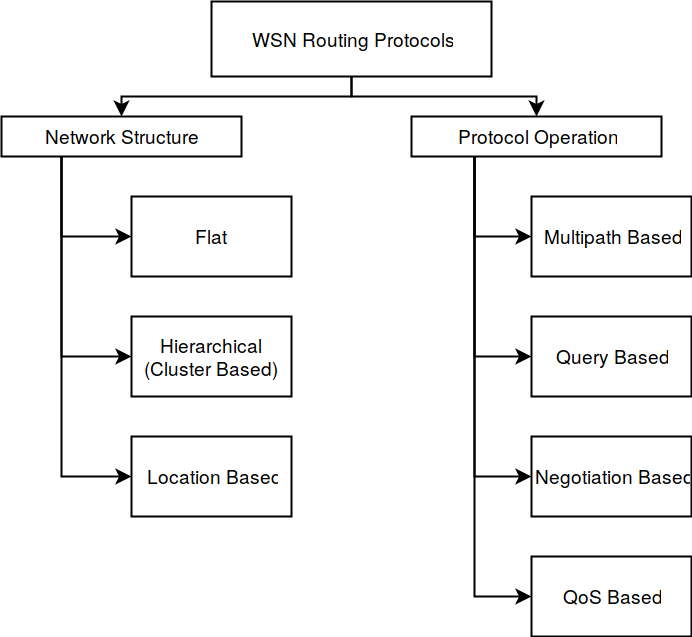
\includegraphics[width=\textwidth]{taxonomy.png}
\caption{Figure showing taxonomy of routing protocols in WSNs.}
\label{fig:taxonomy}
\end{figure}

\section{Routing Protocols in WSNs}
\subsection{Flat-based Routing}
In flat-based routing...

\begin{itemize}
\item SPIN
\item Direct diffusion
\item Rumor routing
\item MCFA 
\item COUGAR
\item ACQUIRE
\item Energy-Aware routing
\end{itemize}


\subsection{Hierarchical Routing}
Hierarchical routing is a well know technique for network routing with special advantages related to scalability, efficient communication and energy-efficient routing in WSNs \cite{leach}\cite{leach_perf}.

\textit{Hierarchical routing is an efficient way to lower energy consumption within a cluster, performing data aggregation and fusion in order to decrease the number of transmitted messages to the base station.}

\begin{itemize}
\item LEACH
\item HEED
\item PEGASIS
\item TEEN/APTEEN
\end{itemize}

\subsection{Location-based Routing}
In location-based routing are the nodes addressed by means of their locations. The distance between neighboring nodes can for example be estimated on the basis of incoming signal strengths or the location of the nodes can be available by using \cite{routing_survey}. 

\begin{itemize}
\item GAF
\item GEAR
\item MFR, DIR, GEDIR
\item SPAN
\end{itemize}

\section{Routing Protocol Operations}
\subsection{Multipath Routing Protocol}
\subsection{Query-based Protocol Operation}
\subsection{Negotiation-based Protocol Operation}
\subsection{QoS-based Protocol Operation}
\subsection{Coherent-based Protocol Operation}
\fi

\chapter{Related Work}
\iffalse
\begin{itemize}
\item Disconnected Operations in the Coda File System
\item Satyanarayanan eller Satya..
\item Energy-efficient communication protocol for wireless microsensor networks - LEACH (2000)
\item Ad-hoc on-demand distance vector routing (1999)
\item Søk etter: sensor networks, sensor net wireless, multipath, leaders, overlay network, overlay, content delivery (CDN)
\end{itemize}
\fi

%\section{Routing Protocols in WSNs}
Wireless sensor networks main task is to periodically collect information of the interested area and broadcast the information to a \gls{bs}. An easy approach to achieve this task is to make each sensor node transmit their data directly to the BS. But the problem  is that the BS can be far away from the sensor node and the sensor node will die due to energy consumption. LEACH, PEGASIS, TEEN and APTEEN are different hierarchical protocols that has been proposed as solutions to this problem \cite{fuzzy_rule}\cite{tree_based}.

LEACH \cite{leach} introduce a hierarchical clustering algorithm for sensor networks. It is self-organized and use randomization to distribute the energy load evenly among the sensors in the network. The sensor nodes  organize themselves into local clusters where one node is the local \gls{bs} or \gls{ch}. The \gls{ch} are not fixed to avoid nodes to drain their battery and to spread the energy usage over multiple nodes. The nodes self-elect a new \gls{ch} depending on the amount of energy left at the nodes at different time-intervals. LEACH is divided into different rounds where each round include a setup phase and a steady-state phase \cite{tree_based}. In the setup phase will each node decide whether to become a \gls{ch} or not. When a \gls{ch} is chosen, each node will select its own \gls{ch} based on the distance between the node and the \gls{ch} and join the cluster. In the steady-state phase will the \gls{ch} fuse the received data from the node members in the cluster and send it to \gls{bs}.

PEGASIS is a chain-based protocol with the idea to form a chain among the sensor nodes so each node will receive from and transmit to a close neighbor. The sensor nodes will also take turns on being the leader for transmitting data to the \gls{bs} and therefor distribute the energy load evenly among the sensor nodes. The chain can be organized by the nodes themselves using a greedy algorithm starting from some node or the \gls{bs} can compute the chain and broadcast it to all the nodes in the network \cite{pegasis}.

Fuzzy logic is also a suitable problem-sovling control system methodologi \cite{fuzzy_logic}.

\Gls{ch} were elected by the \gls{bs} in each round by calculating the change each node has to become the \gls{ch} using three fuzzy descriptors \cite{ch_fuzzy}.
%present some fuzzy logic based clustering protocols .


%\subsection{Hierarchical Routing}
%\subsection{Location-based Routing}
%\subsection{Flat-based Routing}


\chapter{Architecture}
Tell it clean/neat. Abstractions, functionalities


\chapter{Design}
Server, p2p, protocols..

\iffalse
\definition{Another definition}

\begin{table}
\centering
\begin{tabular}{|l|l|}
\hline
Content left & Content right\\
\hline
\end{tabular}
\caption{A table}
\end{table}

\begin{table}
\centering
\begin{tabular}{|l|l|}
\hline
Content left & Content right\\
\hline
\end{tabular}
\caption{Another table}
\end{table}

\newpage

\begin{lstlisting}[frame=single,caption={Small C program},language=C]
#include "stdio.h"
#define e 3
#define g (e/e)
#define h ((g+e)/2)
#define f (e-g-h)
#define j (e*e-g)
#define k (j-h)
#define l(x) tab2[x]/h
#define m(n,a) ((n&(a))==(a))

long tab1[]={ 989L,5L,26L,0L,88319L,123L,0L,9367L };
int tab2[]={ 4,6,10,14,22,26,34,38,46,58,62,74,82,86 };

main(m1,s) char *s; {
  int a,b,c,d,o[k],n=(int)s;
  if(m1==1){ char b[2*j+f-g]; main(l(h+e)+h+e,b);
    printf(b); }
  else switch(m1-=h){
    case f:
      a=(b=(c=(d=g)<<g)<<g)<<g;
      return(m(n,a|c)|m(n,b)|m(n,a|d)|m(n,c|d));
    case h:
      for(a=f;a<j;++a)
        if(tab1[a]&&!(tab1[a]%((long)l(n))))
          return(a);
    case g:
      if(n<h)return(g);
      if(n<j){n-=g;c='D';o[f]=h;o[g]=f;}
      else{c='\r'-'\b';n-=j-g;o[f]=o[g]=g;}
      if((b=n)>=e)
        for(b=g<<g;b<n;++b)o[b]=o[b-h]+o[b-g]+c;
      return(o[b-g]%n+k-h);
    default:
      if(m1-=e) main(m1-g+e+h,s+g); else *(s+g)=f;
      for(*s=a=f;a<e;) *s=(*s<<e)|main(h+a++,
      (char *)m1);
    }
}
\end{lstlisting}

\fi


\chapter{Implementation}
Threads, data structures, language

This chapter will elaborate on how we implemented the system, general implementation requirements, issues and choices. 
%We will first look at some libraries used in this implementation, then we will take a look at ... At last, we will describe the ...

The system is implemented in the open source programming language GO 1.9.3\footnote{\url{https://golang.org/}}.


\chapter{Evaluation}
This chapter describes the experimental setup and metrics used to evaluate the implemented system.

\section{Experimental Setup}
All experiments were done on a Lenovo ThinkCenter with the following specifications:
\begin{itemize} 
\item Intel® CoreTM i5-6400T CPU @ 2.20GHz × 4
\item Intel® HD Graphics 530 (Skylake GT2)
\item 15,6 GiB memory and 503 GB disk
\item Ubuntu 17.04 64-bit with gcc V6.3.0 compiler and GO 1.9.3
\end{itemize}


\section{Experimental Design}
How did we do the experiments?

%For hvert eksperiment bør du prøve å få fram: 
%- hva ønsker du å finne ut? 
%- hvordan måler du + hva måler du? 
%- hva gjør den delen av systemet som du måler? (leser fra disk, regner, sammenligner, koordinerer med andre osv)
%- Hva er metrikken (eks: operasjoner per sekund, minutter per oppgave osv)
%Det gjør det lettere for leseren å henge med. 

%\subsection{Network lifetime?}

\section{Results}
What does the results say?
\subsection{Result 1}
\subsection{Result 2}
\subsection{Result 3}


\chapter{Discussion}
Idea, arch, design, resutls, other solutions, "arch has scale issue"..

This chapter discusses our approach, experience, how we solved the problem and why we chose the solution we ended up with...

\chapter{Conclusion}
In this thesis, we have implemented a system/prototype...

Our experiments showed that the system ...
\chapter{Future Work}

\chapter{Appendix}


\backmatter

%%% BIBLOGRAPHY

\newpage{}

\begin{thebibliography}{9}
%1
\bibitem{leach}
W. R. Heinzelman and A. Chandrakasan and H. Balakrishnan,
\newblock {\em Energy-efficient communication protocol for wireless microsensor networks}, 2000,
\newblock in {\em Proceedings of the 33rd Annual Hawaii International Conference on System Sciences, 10 pp. vol.2-}.

%2 - ikke printet ut
\bibitem{leach_perf}
K. Latif and M. Jaffar and N. Javaid and M. N. Saqib and U. Qasim and Z. A. Khan,
\newblock {\em Performance Analysis of Hierarchical Routing Protocols in Wireless Sensor Networks}, 2012,
\newblock in {\em 2012 Seventh International Conference on Broadband, Wireless Computing, Communication and Applications, pp. 620-625}.

%3
\bibitem{fuzzy_rule}
K. Gotefode and K. Kolhe,
\newblock {\em Energy efficiency in wireless sensor network using Fuzzy rule and tree based routing protocol}, 2015,
\newblock in {\em 2015 International Conference on Energy Systems and Applications, pp. 712-717}.

%4
\bibitem{tree_based}
Z. Han and J. Wu and J. Zhang and L. Liu and K. Tian,
\newblock {\em A General Self-Organized Tree-Based Energy-Balance Routing Protocol for Wireless Sensor Network}, 2014,
\newblock in {\em IEEE Transactions on Nuclear Science Vol.61, Nr.2, pp. 732-740}.

%5
\bibitem{routing_survey}
J. N. Al-Karaki and A. E. Kamal,
\newblock {\em Routing techniques in wireless sensor networks: a survey}, 2004,
\newblock in {\em IEEE Wireless Communications Vol.11, Nr.6, pp. 6-28}.

%6
\bibitem{pegasis}
S. Lindsey and C. S. Raghavendra,
\newblock {\em PEGASIS: Power-efficient gathering in sensor information systems}, 2002,
\newblock in {\em Proceedings, IEEE Aerospace Conference Vol.3, pp. 3-1125-3-1130}.

%7 - ikke skrevet ut
\bibitem{atyp_routing}
X. Liu,
\newblock {\em Atypical Hierarchical Routing Protocols for Wireless Sensor Networks: A Review}, 2015,
\newblock in {\em IEEE Sensors Journal Vol.15, Nr.10, pp. 5372-5383}.

%8
\bibitem{fuzzy_logic}
A. K. Mishra and R. Kumar and J. Singh,
\newblock {\em A review on fuzzy logic based clustering algorithms for wireless sensor networks}, 2015,
\newblock in {\em 2015 International Conference on Futuristic Trends on Computational Analysis and Knowledge Management (ABLAZE), pp. 489-494}.

%9
\bibitem{ch_fuzzy}
Indranil Gupta and D. Riordan and Srinivas Sampalli,
\newblock {\em Cluster-head election using fuzzy logic for wireless sensor networks}, 2005,
\newblock in {\em 3rd Annual Communication Networks and Services Research Conference (CNSR'05), pp. 255-260}.





\end{thebibliography}


\end{document}

